\chapter{Exploration Analytics Methodology}\label{ch3:expl_methods}

\section{Exploration Data Sources}\label{ch3:expl_data_src}

This investigation brings together a total of twenty-five (25) data sets covering the southwest NM study area. Data were collected from previously published works, open-access databases, or derived from those original sources as secondary products. The form of the data varies between pre-gridded raster files, point data sets with repeat or overlapping measurements, non-overlapping point sets, and line data. Previous researchers created raster files or raster-ready gridded data for nine of the features. Four are generated by running procedures on one of the existing rasters. The remaining layers were created from polylines (3), overlapping points (4), and non-overlapping points (2). Although complex interactions between earth systems should be expected, these layers represent the independent variables for analysis purposes. Section XXX details how evaluating collinearities between features allows for pre-screening before modeling, and further analysis of feature importances helps reduce this composite data set to a smaller subset for simpler prediction models.

\begin{table}[htp]
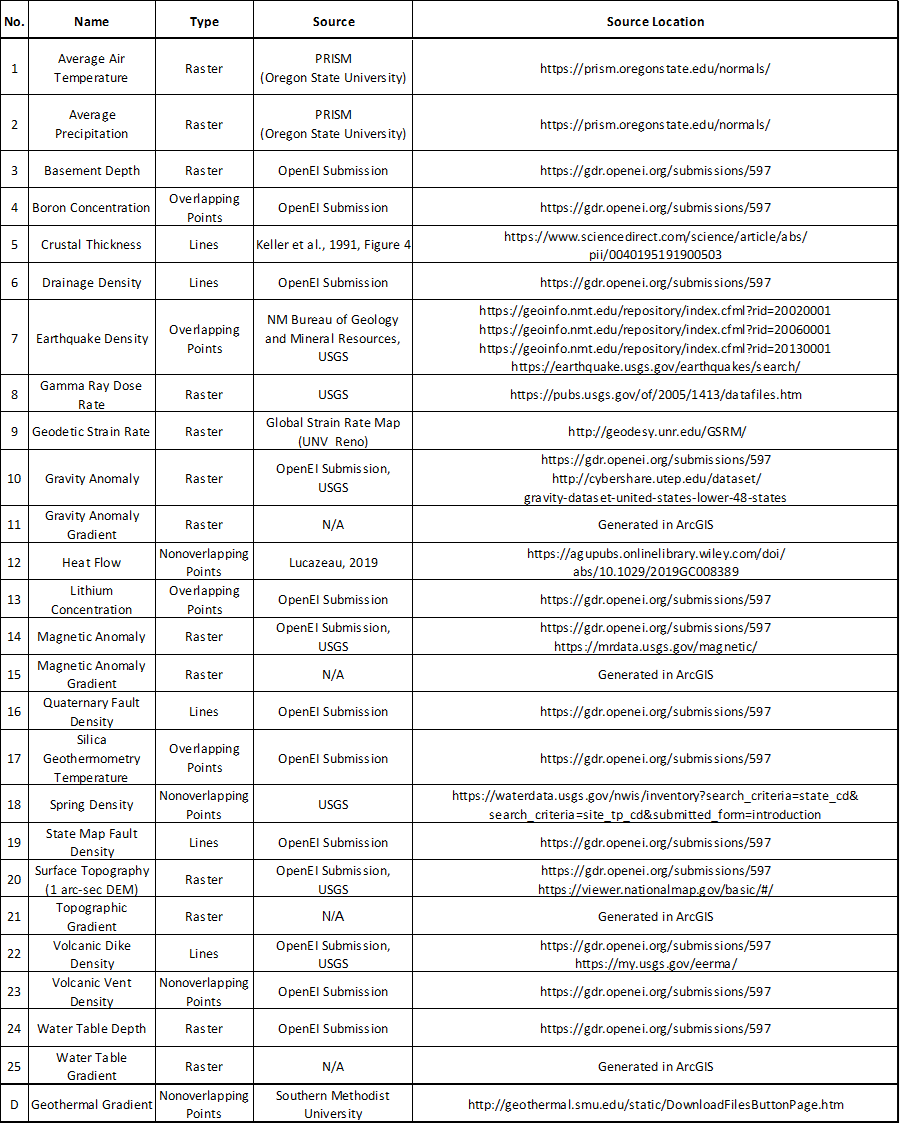
\includegraphics[scale=1.9]{Table-Features.png}
\caption[Features considered in this the exploration analytics study]{List of data sets considered in this study. Data type, provider, and source location are listed. Numbered features are treated as independent variables. 'D' indicates the dependent variable.}
\label{tab:features}
\end{table}

As discussed in Section \ref{ch2:sysfund}, geothermal systems require permeability, heat, subsurface fluids, a trapping mechanism, and recharge. Following the slightly more simplified PFA assumptions of \citeauthor{bielicki_hydrogeolgic_2015} (\citeyear{bielicki_hydrogeolgic_2015}), an explorationist will want to quickly identify where heat, permeability, and fluids together define a favorable setting for a geothermal prospect. The prepared independent data inputs collectively address all three elements as noted in Table xx. Rather than defining a dependent (predicted) variable that describes a total favorability score, this thesis focuses on a proof of concept prediction for a measurable quantity addressing just the heat risk element: geothermal gradient. This choice was made because a) geothermal gradient provides a direct proxy for accessible heat content, b) gradient point data is available from suitable compilations of well measurements collected across the study area, and c) for EGS applications, the only risk element that must be naturally present is heat. Heat flow might be a reasonable alternative dependent variable, however point values for heat flow in the available well database were derived directly from geothermal gradient values. Geothermometer measurements also suggest resource temperatures, but the uncertainty in fluid pathways leading to the sample location means these values suffer from less spatial and depth certainty than geothermal gradient.

Regarding the remaining two risk elements: direct measurements of permeability (i.e., from downhole logs or core analysis) or fluids (e.g., flow rate from well tests) can be separately predicted using the same methods described in this study. A final favorability score, which is less straight-forward to calibrate for model validation and verification, could potentially be derived from the combined predictions as done in PFA risk assessments. This suggestion is outside of the scope of this thesis and thus appears in the list of future work opportunities (see Chapter 9).

\section{Exploration Data Preparation}

\subsection{Digital Elevation Map}
